%!TEX root = ../rapport.tex

\renewcommand{\abstractname}{Auteur du document}
\begin{abstract}

\begin{tabular}{m{9.5cm}m{0.8cm}m{3.8cm}}
	Etudiant en troisième et dernière année de l'\emph{\gls{eiafr}} en section informatique, ce travail clôture mon cursus scolaire et sera l'étape finale me permettant d'obtenir un \emph{Bachelor of Science in Computer Science}. 

	\medskip 

	Etant un grand passioné des technologies du \emph{web} et mobiles, ce projet m'a tout de suite attiré tant pour sa partie développement \emph{\gls{ios}} que celle du \emph{\gls{webservice}}.
	&&\multirow{2}{3.8cm}{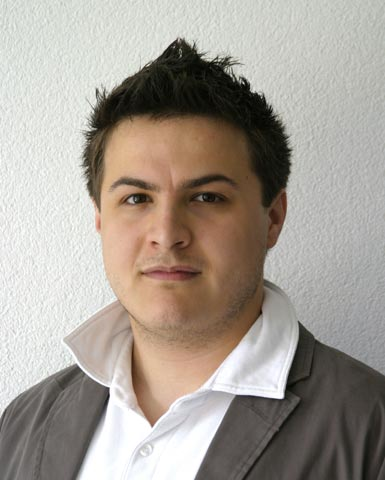
\includegraphics[width=3.8cm]{01_Introduction/media/photo_passeport_20.jpg}}\\
 	 
 	\vspace{0.5cm}

 	\textbf{Ingénierie d'application}  : Java, JR, Adobe AIR - FLEX, ActionScript, C, C++&&\\
 	\vspace{0.2cm}
 	\textbf{Développement Web} : PHP, HTML 4/5, CSS 2/3, Xataface, Contao, Joomla, Drupal, JSF / JSP, Adobe FLEX, ActionScript, Java EE&&\\
 	\vspace{0.2cm}
 	\textbf{Développement mobile} : IOS, Android&&\\
 	\vspace{0.2cm}
 	\textbf{Gestion des données} : MySQL, SQLite, Access, Oracle, SQLServer, technologies XML&&\\
\end{tabular}

\end{abstract}